\section{Méthodologie de la recherche}
\subsection{ Présentation des données }
\subsubsection{Données brute}
\par{
Les données que nous utilisont dans cette étude proviennent du site web investing.com.
Il s'agit des données de cours journalière des indices : }
\begin{itemize}
\item[$\diamond$] BRVM-Agriculture 
\begin{table}[ht]
	\rowcolors{2}{myblue}{white}
	\centering
	\caption{Présentation des données de la BRVM-Agriculture}\label{tab:multirow}
	\begin{tabular}{p{2cm}p{2cm}p{2cm}p{2cm}p{2cm}p{2cm}}
		\hline
		Date 		& Dernier 	& Ouv 		& Plus Haut & Plus Bas 	& Variation\%	\\
		\hline                                                                  
		29/11/2021  &247,95  &244,32     &248,97   &244,32       &1,49\%    \\
		30/11/2021  &248,36  &247,95     &248,43   &247,95       &0,17\%  	\\
		01/12/2021  &249,12  &248,36     &250,45   &248,36       &0,31\%    \\
		02/12/2021  &250,05  &249,12     &251,09   &250,05       &0,37\%    \\
		03/12/2021  &243,92  &250,05     &250,05   &243,92      &-2,45\%    \\
		...            &...     &...        &...      &...         &...     \\
		09/05/2023  &260,09  &263,37     &263,37   &260,09      &-1,25\%   	\\
		10/05/2023  &253,34  &260,09     &263,07   &247,71      &-2,60\%    \\
		11/05/2023  &251,77  &253,34     &254,20   &243,82      &-0,62\%    \\
		12/05/2023  &249,87  &251,77     &253,49   &243,25      &-0,75\%   	\\
		15/05/2023  &248,05  &249,87     &250,58   &243,85      &-0,73\%  	\\
		\hline
	\end{tabular}
\end{table}%

\item[$\diamond$] BRVM-Services publics
\begin{table}[ht]
	\rowcolors{2}{myblue}{white}
	\centering
	\caption{Présentation des données de la BRVM-Service Public}\label{tab:multirow}
	\begin{tabular}{p{2cm}p{2cm}p{2cm}p{2cm}p{2cm}p{2cm}}
		\hline
		Date 		& Dernier 	& Ouv 		& Plus Haut & Plus Bas 	& Variation\%	\\
		\hline                                                                        
		26/11/2021  &440,30  &440,62     &445,25   &440,30      &-0,07\% \\ 
		29/11/2021  &442,39  &440,30     &449,47   &440,30      &0,47\%    \\ 
		30/11/2021  &450,26  &442,39     &450,36   &442,39      &1,78\%  \\   
		01/12/2021  &449,67  &450,26     &450,26   &449,67      &-0,13\%  \\   
		02/12/2021  &449,50  &449,67     &450,09   &449,50      &-0,04\%  \\   
		...           & ...     &...       & ...     & ...       &  ...     \\   
		09/05/2023  &481,66  &479,45     &481,76   &478,08       &0,46\%  \\   
		10/05/2023  &482,27  &481,66     &492,36   &479,30       &0,13\%  \\   
		11/05/2023  &486,77  &482,27     &486,77   &480,22       &0,93\%  \\   
		12/05/2023  &489,95  &486,77     &490,69   &483,95       &0,65\%  \\   
		15/05/2023  &468,96  &489,95     &489,95   &459,94      &-4,28\%  \\   
		\hline
	\end{tabular}
\end{table}%
\end{itemize}

\newpage

\subsubsection{Données pré-traité}

\textbf{Stratégie des Moyennes Mobiles.}
\begin{samepage}
\begin{table}[ht]
\rowcolors{2}{myblue}{white}
\centering
\caption{Données Pré-traités pour la stratégie des Moyennes Mobiles pour l'indice BRVM-Agriculture}\label{tab:multirow}
\begin{tabular}{p{2cm}p{2cm}p{2cm}p{2cm}p{2cm}p{1.5cm}}
	\hline
	Date 		&Dernier &Ouv 	&Variation	&MA26 		& MA61	\\ 
	\hline                                                                  
	03/09/2020	&65,30	&67,55	&-3,33\%	&60,16	&61,63  \\ 
	04/09/2020	&65,42	&65,30	&0,18\%		&60,50	&61,63  \\ 
	07/09/2020	&65,35	&65,42	&-0,11\%	&60,91	&61,65  \\ 
	08/09/2020	&66,64	&65,35	&1,97\%		&61,37	&61,69  \\ 
	09/09/2020	&66,83	&66,64	&0,29\%		&61,84	&61,75  \\
	...			&...	&	...	&	...		&...		&... \\ 
	09/05/2023	&260,09	&263,37	&-1,25\%	&275,57	&284,27   \\
	10/05/2023	&253,34	&260,09	&-2,60\%	&274,15	&283,54   \\
	11/05/2023	&251,77	&253,34	&-0,62\%	&272,80	&282,78   \\
	12/05/2023	&249,87	&251,77	&-0,75\%	&271,32	&281,95   \\
	15/05/2023	&248,05	&249,87	&-0,73\%	&269,76	&281,12 \\
	\hline
\end{tabular}
\end{table}%

\begin{table}[ht]
\rowcolors{2}{myblue}{white}{white}
\centering
\caption{Données Pré-traités pour la stratégie des Moyennes Mobiles pour \\l'indice BRVM-Service Public}\label{tab:multirow}
\begin{tabular}{p{2cm}p{2cm}p{2cm}p{2cm}p{2cm}p{1.5cm}}
	\hline
	Date 		&Dernier &Ouv 	&Variation	&MA48 		& MA98 \\ 
	\hline                                                                  
	03/11/2020	&355,67	&370,36	&-3,97\%	&360.05	&373.16 \\ 
	04/11/2020	&357,55	&355,67	&0,53\%		&359.51	&372.76 \\ 
	05/11/2020	&361,29	&357,55	&1,05\%		&359.04	&372.38 \\ 
	06/11/2020	&358,76	&361,29	&-0,70\%	&358.61	&372.01 \\ 
	09/11/2020	&357,66	&358,76	&-0,31\%	&358.16	&371.64 \\ 
	...			&...	&...	&...		&...		&... \\ 
	09/05/2023	&481,66	&479,45	&0,46\%		&487.29	&486.53  \\
	10/05/2023	&482,27	&481,66	&0,13\%		&487.08	&486.74  \\
	11/05/2023	&486,77	&482,27	&0,93\%		&486.88	&487.00  \\
	12/05/2023	&489,95	&486,77	&0,65\%		&486.70	&487.29  \\
	15/05/2023	&468,96	&489,95	&-4,28\%	&485.98	&487.37 \\
	\hline
\end{tabular}
\end{table}%
\end{samepage}

\newpage

\begin{samepage}
\textbf{Stratégie Combiné de l'Oscillateur Stochastique et de}\\
\textbf{ la moyenne Mobile Convergence Divergence. }

	\begin{center}
	\begin{table}[ht]
		\rowcolors{2}{myblue}{white}
		\centering
		\caption{Données Pré-traités pour la stratégie Combiné de 
		l'Oscillateur Stochastique et de la moyenne Mobile Convergence Divergence 
		pour l'indice BRVM-Agriculture}\label{tab:multirow}
		\begin{tabular}{p{1.5cm}p{1cm}p{1.5cm}p{1cm}p{1cm}p{1cm}p{1cm}p{1.5cm}p{1.5cm}p{1.5cm}}
			\hline
			Date 		&Dern.	&Ouv.	&Haut	&Bas	&\%k	&\%d	&MACD(10,25)	&Signal(4)	&Hist \\ \\
			\hline                                                                  
			15/07/2020	&60,14	&62,33	&62,33	&60,14	&0.00	&0.00	&-0.925	&-0.56	&-0.36 \\ 
			16/07/2020	&59,09	&60,14	&60,14	&59,09	&0.00	&0.00	&-1.290	&-0.85	&-0.43	\\
			17/07/2020	&58,41	&59,09	&59,09	&58,41	&0.00	&0.00	&-1.618	&-1.15	&-0.45\\ 
			20/07/2020	&57,05	&58,41	&58,41	&57,05	&0.00	&0.00	&-1.986	&-1.49	&-0.49\\ 
			21/07/2020	&57,05	&57,05	&57,18	&57,05	&0.00	&0.00	&-2.236	&-1.78	&-0.44\\
			...			&...	&...	&...	&...	&...	&...	&...	&...	&... \\ 
			09/05/2023	&260,09	&263,37	&263,37	&260,09	&12.02	&20.15	&-7.143	&-6.79	&-0.34 \\
			10/05/2023	&253,34	&260,09	&263,07	&247,71	&15.53	&16.97	&-7.970	&-7.26	&-0.70 \\
			11/05/2023	&251,77	&253,34	&254,20	&243,82	&19.81	&15.79	&-8.648	&-7.81	&-0.82\\ 
			12/05/2023	&249,87	&251,77	&253,49	&243,25	&16.29	&17.21	&-9.238	&-8.38	&-0.85\\ 
			15/05/2023	&248,05	&249,87	&250,58	&243,85	&12.14	&16.08	&-9.745	&-8.93	&-0.81 \\
			\hline
		\end{tabular}
	\end{table}%
	\newpage
	\begin{table}[ht]
		\rowcolors{2}{myblue}{white}
		\centering
		\caption{Données Pré-traités pour la stratégie Combiné de 
		l'Oscillateur Stochastique et de la moyenne Mobile Convergence Divergence
		pour l'indice BRVM-Service Public}\label{tab:multirow}
		\begin{tabular}{p{1.5cm}p{1cm}p{1.5cm}p{1cm}p{1cm}p{1cm}p{1cm}p{1.5cm}p{1.5cm}p{1.5cm}}
			\hline
			Date 		&Dern.	&Ouv.	&Haut	&Bas	&\%k	&\%d	&MACD(25,36)	&Sigal(6)	&Hist \\	\\
			\hline                                                       
			13/07/2020	&382,46	&383,01	&383,08	&382,46	&0.00	&0.00	&-1.19	&-0.79	&-0.40 \\ 
			14/07/2020	&382,66	&382,46	&382,66	&382,46	&1.15	&0.38	&-1.35	&-0.95	&-0.39\\ 
			15/07/2020	&382,32	&382,66	&383,27	&382,32	&0.00	&0.38	&-1.49	&-1.11	&-0.38\\ 
			16/07/2020	&380,34	&382,32	&383,53	&380,34	&0.00	&0.38	&-1.65	&-1.26	&-0.39\\ 
			17/07/2020	&384,42	&380,34	&384,42	&380,34	&20.96	&6.98	&-1.69	&-1.38	&-0.30\\ 
			...	&...	&...	&...	&...	&...	&...	&...	&...	&... \\ 
			09/05/2023	&481,66	&479,45	&481,76	&478,08	&90.70	&86.27	&-1.57	&-1.77	&0.19\\ 
			10/05/2023	&482,27	&481,66	&492,36	&479,30	&68.53	&80.18	&-1.45	&-1.68	&0.22\\ 
			11/05/2023	&486,77	&482,27	&486,77	&480,22	&82.56	&80.60	&-1.23	&-1.55	&0.32\\ 
			12/05/2023	&489,95	&486,77	&490,69	&483,95	&92.48	&81.19	&-0.96	&-1.38	&0.42\\ 
			15/05/2023	&468,96	&489,95	&489,95	&459,94	&27.82	&67.62	&-1.20	&-1.33	&0.13\\ 
			\hline
		\end{tabular}
	\end{table}%
\end{center}
\end{samepage}		


\subsection{Méthode, outils de collecte de pré-traitement et de traitements des données} 
\subsubsection{Méthode de collecte des données}
\par{Les données de cette étude ont été collectées sur la plateforme investing.com qui 
est une plateforme d'informations et d'actualités sur les marchés financiers 
fournissant des données en temps réel, des cotations, des graphiques, des outils
financiers, des informations de dernière minute et des analyses sur 250 marchés
boursiers du monde entier dans 44 éditions internationales. C'est l'un des trois premiers sites
Web financiers mondiaux au monde.}	

\subsubsection{Outils de traitement des données}
\par{
Notre étude à été réalisé en utilisant le langage de proagrmmation python, grâce aux environnements 
de développement Visual Studio Code et Jupyter Notebook.}

\begin{itemize}
	\item[$\bullet$] 
\includegraphics[height=1em]{icons/python-icon.jpg} Python
	\par{Python est un langage de programmation interprété multiparadigme et multiplateforme.}

	\item[$\bullet$] 
\includegraphics[height=1em]{icons/vscode-icon.png} Visual Studio Code
	\par{Visual Studio Code est un éditeur de code open-source et gratuit développé 
		par Microsoft. Il prend en charge plusieurs langages de programmation et 
		possède à cet effet une grande variété d'extensions afin de faciliter le 
		travail du développeur.}

	\item[$\bullet$] 
\includegraphics[height=1em]{icons/jupyter-icon.png} Jupyter Notebook
	\par{
		Jupyter Notebook est une application web qui permet de créer et partager 
		des documents informatiques. Il offre une expérience simple, rationalisée 
		et centrée sur les documents. Jupyter prend en charge plusieurs langages 
		de programmation, notamment Python, R et Julia.}

\end{itemize}

\begin{center}	Bibliothèque utilisées \end{center} 
\begin{itemize}
	\item[$\bullet$] 
\includegraphics[height=1em]{icons/pandas-icon.png} Pandas
	\par{Pandas est un package Python qui fournit des structures de données rapides,
	flexibles et expressives conçues pour rendre le travail avec des données 
	"relationnelles" ou "étiquetées" à la fois simple et intuitif. Il vise à être 
	le bloc de construction fondamental de haut niveau pour effectuer une analyse 
	pratique et réelle des données du monde en Python.}

	\item[$\bullet$] 
\includegraphics[height=1em]{icons/numpy-icon.png} NumPy
	\par{Largement utilisée pour le calcul scientifique et numérique, NumPy fournit 
	des structures de données et des fonctions optimisées pour manipuler des 
	tableaux multidimensionnels, ce qui en fait un outil puissant pour le traitement 
	des données. NumPy est le package fondamental pour le calcul scientifique avec Python.}

	\item[$\bullet$] 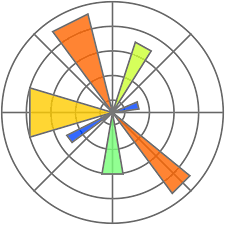
\includegraphics[height=1em]{icons/matplotlib-icon.png} Matplotlib
	\par{Matplotlib est une bibliothèque complète pour créer des visualisations statiques, 
	animées et interactives en Python.}
\end{itemize}

\begin{center}	Formule Statistique \end{center} 

\textbf{Moyenne Mobile Arithmetique}
\par{On appelle moyenne mobile centrée d'ordre k de la série $\{Y_t, t=1,\ldots,n\}$ les
Moyennes Mobiles arithmétiques calculées sur $k$ valeurs successives.}
\begin{itemize}
\item[$\diamond$] Si  k est impaire avec k=2m+1 :\\ 
\large{$M_{t}(k)$ = $\frac{1}{k}\sum_{i=m}^{m}Y_{t+i}$}
\item[$\diamond$] Si  k est paire avec k=2m :\\
\large{$M_t(k)$ = $\frac{1}{k}\left[\frac{Y_{t-m}}{2}+ \sum_{i=-m+1}^{m-1}Y_{t+i} + \frac{Y_{t+m}}{2}\right]$ }\\
% + \sum_{i=-m+1}^m-1 + \fact{Y_{t+m}}{2} 
\end{itemize}


\textbf{Moyenne Mobile Exponentielle}
\begin{itemize}
\item[$\diamond$] Formule de la Moyenne Mobile Exponentielle: \\
\begin{equation}
	\large{\bar{x}_t = \alpha\left( x_t + \left(1 - \alpha \right)x_{t-1} + {\left(1 - \alpha \right)}^2x_{t-2} + {\left(1 - \alpha \right)}^3x_{t-3} + \ldots \right)}
\end{equation}
\begin{equation}\large{\bar{x}_t = \sum_{n=0}^{\infty}\alpha{\left(1 - \alpha\right)}^nx_{t-n} } \end{equation}
\end{itemize}	

\textbf{Oscillateur Stochastiue} 
\begin{itemize}
\item[$\diamond$] Formule de la ligne \%K sur une période p:

\item[$ $] $\%K$ = ${\frac{(C - L)}{(H - L)}}*100$
\item[--] C : c'est le prix de clôture de l'actif.
\item[--] L : c'est le prix le plus bas de l'actif sur les N dernères périodes.
\item[--] H : c'est le prix le plus élevé de l'actif sur les N dernière périodes\\
\begin{large}
\begin{equation}
	\begin{cases}
		\large{L = Y_{min_t}  = min\left( Y_{t-p},Y_{t-p+1},\ldots,Y_{t+p} \right)}\\
		\\
		\large{H = Y_{max_t} = max\left( Y_{t-p},Y_{t-p+1},\ldots,Y_{t} \right)}
		%\item[$ $] $L = Y_{min_t} = min\left( Y_{t-p},Y_{t-p+1},\ldots,Y_{t+p} \right)$\\
		%\item[$ $] $H = Y_{max_t} = max\left( Y_{t-p},Y_{t-p+1},\ldots,Y_{t+p} \right)$
	\end{cases}
\end{equation}
\end{large}
\item[$\diamond$] Formule de la ligne $\%D$
\item[--] Si k est impaire : \begin{large} $\%D_t(k)$ = $\frac{1}{k}\sum_{i=m}^{m}\%K_{t+i}$\end{large}  \\
\item[--] Si k est paire : \begin{large}$\%D_t(k)$ = $\frac{1}{k}\left[\frac{\%K_{t-m}}{2}+ \sum_{i=-m+1}^{m-1}\%K_{t+i} + \frac{\%K_{t+m}}{2}\right]$\end{large}\\


\end{itemize}


\textbf{Moyenne Mobile Convergence Divergence} 

\begin{itemize}
\item[$\diamond$] Formule de la MACD\\
Soit C et L les périodes respectives des Moyennes Mobiles rapide et des Moyennes Mobiles lente.

	\begin{large}
		\begin{equation}
			macd = \bar{x}_C(t)-\bar{x}_L(t)
		\end{equation}
		\begin{equation}
			\begin{cases}
				\bar{x}_t(C) = 
					\sum_{n=0}^{C}\alpha{\left(1 - \alpha\right)}^nx_{t-n}\\

				\bar{x}_t(L) = 
					\sum_{n=0}^{L}\alpha{\left(1 - \alpha\right)}^nx_{t-n}
			\end{cases}
		\end{equation}
	\end{large}

%$\alpha x_{t}+(1-\alpha)\bar{x}_{t-1} $ - $\alpha x_{t} + (1-\alpha)\bar{x}_{t-1} $

\item[$\diamond$] Formule de la ligne SIGNALE
Soit S la période de la moyenne mobile de la ligne SIGNALE
\begin{equation}
	\begin{cases}
	\text{Si S est impaire}:\begin{large} \%D_t(k) = \frac{1}{S}\sum_{i=m}^{m}macd_{t+i}\end{large}\\ 
	\text{Si S est paire} : \begin{large} \%D_t(k) = \frac{1}{S} \left[\frac{macd_{t-m}}{2}+ \sum_{i=-m+1}^{m-1}\%K_{t+i}+ \frac{\%K_{t+m}}{2} \right] \end{large}
	\end{cases}
\end{equation}

\end{itemize}



\subsection{Profil d'investisseur et paramètres des stratégies de traing.}
\par{
Pour déterminer qu'une stratégie est meilleur pour un indice précis nous devons d'abord déterminer 
les bons paramètres qui maximise le rendement de la stratégie.
La détermination des meilleurs paramètres pour chaque stratégies passe par une étape de validation 
durant laquelle les meilleur paramètres devrons respecter un certain nombre de critère de validation 
élaborer dans le cadre de cette étude. Notons également que les critère de validation présenter 
ci-dessous s'adapte à un profil d'investisseur précis dans le cadre de cette étude.}

\subsubsection{Profil d'investissement.}
\par{
Le profil d'investisseur est généralement défini en fonction du niveau de tolérance au risque financier 
qu'un investisseur est prêt à assumer, en comprenant le risque financier comme capacité d'assumer une 
perte. Il est déterminée en évaluant des éléments du caractère de l'investisseur comme la rentabilité 
qu'il espère obtenir, son objectif d'investissement, sa tolérance au risque[2].}



\begin{itemize}
\item[$\diamond$]\textbf{Objectifs d'investissement.}
\par{
Les objectifs d'investissement en trading peuvent varier en fonction des stratégies et 
des préférences de chaque individu ou institution. Voici quelques 
types d'objectifs d'investissement courants en trading :}
\begin{enumerate}
	\item Objectif de croissance du capital ;
	L'objectif principal est de réaliser des profits en augmentant la valeur du 
	capital investi. Les traders cherchent à exploiter les mouvements du marché 
	pour générer des rendements positifs.

	\item Protéger son patrimoine contre un risque donné grâce à une stratégie de couverture ; 
	c'est-à-dire prendre des mesures pour réduire ou neutraliser l'impact des fluctuations 
	défavorables sur la valeur d'un actif ou d'un portefeuille d'investissement. Cette 
	approche est souvent utilisée pour minimiser les pertes potentielles causées par des 
	mouvements de marché indésirables[7].
	
	\item Spéculer sur les marchés ;  
	c'est-à-dire à faire des paris sur l'évolution des prix à la hausse comme à la 
	baisse[7].

	\item Objectif de revenu régulier : Certains traders cherchent à obtenir un revenu 
	régulier en utilisant des stratégies de trading qui visent à générer des gains 
	constants à partir de leurs investissements.

\end{enumerate}

	\item[$\diamond$]\textbf{Horizon temporel.}
	\par{
		Un horizon temporel (ou un horizon d'investissement) correspond à la durée totale pendant    laquelle un titre est supposé être détenu par un investisseur. 
		Les types d'horizons temporels varient de court terme à long terme. Certains traders fixent 
		un horizon d'investissement plus long car ils disposent de plus de temps pour maintenir 
		leur portefeuille investi et ainsi réaliser des bénéfices ou compenser les pertes subies. 
		Normalement, avec un horizon à long terme, les investisseurs se sentent plus à l'aise pour 
		prendre des décisions d'investissement plus risquées et capitaliser sur la volatilité 
		du marché. Alors qu'à court terme, comme dans le cas d'un trader (négociateur sur séance),
			les investisseurs doivent veiller à éviter les investissements plus risqués (en particulier 
			ceux qui sont proches de l'échéance) afin de ne pas subir de pertes significatives[8].
		Il s'agit ici d'un facteurs crucial qui influence le choix de notre stratégie d'investissement.
		
	
	}
	
	\item[$\diamond$]\textbf{Tolérance au risque.}
	\par{
	En investissements la tolérance au risque est la capacité et la volonté d'un investisseur à 
	assurumer une perte de la valeur de notre placement. }

	\begin{enumerate}
		\item Prudent : 
		La tolérance au risque et la capacité à l'assumer sont toutes deux faibles. 
		Les placements comporteront probablement moins d'actions et plus d'obligations ou 
		d'actifs du marché monétaire (qui procurent généralement des rendements stables et 
		moins de fluctuations de cours)

		\item Modéré : 
		La niveaux modéré traduit une tolérance au risque plutôt élevée, 
		mais une capacité moindre. Ici les placements pourraient comprendre une combinaison 
		d'actions et d'obligations pour une approche plus équilibrée. 

		\item Énergique : 
		Ici votre tolérance au risque est élevée, tout comme votre capacité 
		à prendre des risques. Vous acceptez que la valeur de vos placements puisse 
		subir de grandes fluctuations au fil du temps. Vous rechercherez probablement 
		un potentiel de rendement plus élevé. Vos placements sont probablement 
		composés principalement d'actions (plutôt que d'obligations) de sociétés de 
		grande et de petite taille. 

	\end{enumerate}	
\end{itemize}


\subsubsection{Critères de choix des paramètres.}
\par{
	La Stratégie des Moyennes Mobiles se base sur une étude  des tendances des Moyennes Mobiles de courte périodes 
	et de longue périodes. A cet effet, il existe des périodes standards dans l'utilisation de cette Stratégie. 
	Ces périodes dépendent de divers facteurs, notamment de la volatilité des actifs et de l'horizon 
	temporel (court terme : MA5, MA10, moyen terme : MA50, MA100, long terme : MA200, MA250). 
	Cependant, il est souvent nécessaire d'adapter ces périodes en fonction des conditions changeantes
	du marché et des besoins de l'investisseur.
	De plus la stratégie de l'Oscillateur Stochastique et de la moyenne mobile convergence divergence fait 
	également appelle au calcul de certaine moyenne mobile.
	Ainsi, dans l'application de la Stratégie de trading basée sur les Moyennes Mobiles, et celle de la 
	méthode combiné de l'Oscillateur stochastique et de la moyenne mobile convergence divergence nous avons 
	testé différentes combinaisons qui ont permis de trouver les périodes des Moyennes Mobiles 
	rapide et des Moyennes Mobiles lentes optimales, permettant d'appliquer efficacement la stratégie de trading.
	Il s'avère donc nécessaire de faire un choix logique, cohérent et robuste suivant toutes les
	périodes trouvées, nos objectifs d'investissements, notre horizon temporel et la tolérance au risque.
	
}

\begin{itemize}
	\item[$\diamond$]\textbf{Simulation}
	\par{La simulation consistera à tester plusieurs combinaisons de périodes pour les Moyennes Mobiles 
    arithmétiques dans le cas de la stratégie basée sur les Moyennes Mobiles. Nous allons recueillir des
    informations sur le pourcentage de bénéfice réalisé à la suite du backtesting, 
    le nombre total de signaux d'achat et de vente obtenus
    en utilisant les combinaisons de périodes, le nombre de transactions positives effectuées et le nombre de transactions 
    négatives. Dans le cas de la Stratégie combinée de l'Oscillateur Stochastique et de la moyenne mobile Convergence Divergence, 
    nous allons recueillir des informations sur le bénéfice, le nombre de transactions positives effectuées et le 
    nombre de transactions négatives, ainsi que les combinaisons de périodes utilisées pour calculer les moyennes exponentielles, la ligne de signal et la ligne de l'Oscillateur Stochastique.

    Notre étude encourage l'investissement à cout et à long terme, ainsi donc nos simulations se 
    feront pour des valeurs de la période courte de 20 à 50 et pour des valeurs de la période longue de 50 à 150.
    À la fin de la simulation, nous choisirons les périodes ayant généré un bénéfice d'au moins 20\%, 
    un taux de transactions positives élevé et robuste.


 }


	\item[$\diamond$]\textbf{Taux de réussite des transactions.}
	\par{Une transaction est réussite lorsque le prix d'achat de l'actif est inférieur au prix de ventes.
    En d'autre termes, la transaction est réussite lorsque nous réalisons un bénéfice.
    Il arrive en effet lors de la génération des signaux que l'on obtiennent des faux signaux causé par un retard
    ,une grand fluctuation du marché etc... 
    Le taux de réussites des transaction mesure donc la performance de la combinaison de 
    période utilisée en ce basant sur le nombre de transaction réussi par rapport au nombre total de transactions
    effectuer.
    

}

	\item[$\diamond$]\textbf{Robustesse }
	\par{La Robustesse est la capacité à ne pas être perturbé par une modification dans une petite
    partie des données. Une période est résistante lorsque la rentabilité produite par la période
    n'est pas très éloigner des rentabilités produites par les périodes avoisinantes.}



\end{itemize}


